\Needspace{8\baselineskip}
\section{Affine blocks and exact projection}
\label{offset:section}

We now compress a product scalar-image instance into blocks with
constant-size value spaces. The construction uses \(r\) cyclic address
coordinates and will support simultaneous choices on at most
\(K=r+1\) blocks. Its purpose is to provide compatible affine translations
that can be extended whenever one more block becomes active. The wire subdivision and corner-potential method is shared with
the fixed-dimension companion \citep[Section~3]{CompanionFixedDimension};
we prove the binary, growing-dimension version here, including the
single-readout fullness required by the subcubic realization. The conclusion is the exact restriction equality in
\Cref{prop:exact-projection}, which supplies the choices used by the
Duplicator strategy.

Throughout this section, \(r\geq 3\), \(K=r+1\), and the input is a product
scalar-image instance as in \Cref{def:scalar-images}. The block data are
constructed from that instance alone. Witnessing sets \(Q_{P,\mathbf a}\),
when they exist, will be used only to prove the extension property.

\subsection{Subdivided comparison wires}
\label{offset:subdivision}

Write each affine endpoint form of a comparison schema \(e:P\to R\) as
\[
  \phi_{e,j}(v)=\lambda_{e,j}(v)+c_{e,j},
  \qquad j\in\{0,1\},
\]
where \(\lambda_{e,j}\) is linear and \(c_{e,j}\in\F\).
Replace \(e\) by its own oriented wire
\[
  P=t_0,\ t_1,\ldots,t_{4K},\ t_{4K+1}=R.
\]
The \(4K\) internal types are private to this wire and have value dimension
one. The endpoints are the original real types, with their original
dimensions \(d_P,d_R\in\{1,2\}\). If \(P=R\), the endpoint types are
identified, but the internal types and all \(4K+1\) links remain distinct.
In particular, every individual link has distinct endpoint types. Denote
the resulting set of all types by \(\mathcal T\), and write \(d_t\) for
the value dimension at \(t\in\mathcal T\).

For each coordinate \(i\in\{1,\ldots,r\}\), the allowed labels at a type
are
\[
 A_{t,i}=
 \begin{cases}
   \{0,1\}, & t\text{ is real},\\
   A_{e,i}, & t\text{ is internal to the wire of }e.
 \end{cases}
\]
For a link \(\ell=tu\), oriented toward the second endpoint of its wire,
let \(\cM_{\ell,i}\subseteq A_{t,i}\times A_{u,i}\) be its coordinate
matches. On every link except the last these are
\((a,a)\), \(a\in A_{e,i}\). On the last link they are
\((a,\sigma_{e,i}(a))\), \(a\in A_{e,i}\).
Thus a full address \(\mathbf a\in A_e\) is unchanged along the internal
types and is sent to \(\boldsymbol\sigma_e(\mathbf a)\) at the second real
endpoint.

Associate to every link a scalar equation
\begin{equation}
   L_{\ell,t}h_t+L_{\ell,u}h_u=b_\ell,
   \qquad h_t\in\F^{d_t},\quad h_u\in\F^{d_u}.
   \label{eq:link-equation}
\end{equation}
Here the form at an internal type is the identity. On the first link,
the form at \(P\) is \(\lambda_{e,0}\) and \(b_\ell=c_{e,0}\);
on the last link, the form at \(R\) is \(\lambda_{e,1}\) and
\(b_\ell=c_{e,1}\); on every other link \(b_\ell=0\).
Consequently the first and last equations respectively say
\[
 h_{t_1}=\phi_{e,0}(h_P),
 \qquad
 h_{t_{4K}}=\phi_{e,1}(h_R),
\]
and the interior equations identify all the internal scalars.
This interpretation includes constant endpoint forms. For a loop wire,
the two occurrences of its real endpoint retain their respective forms.

\subsection{Readouts, blocks, and affine fibers}
\label{offset:blocks}

Index boundaries cyclically by \(i\in\{1,\ldots,r\}\), so that \(r+1\)
means \(1\), and put
\[
 \delta_i=
 \begin{cases}
  1,&i=r,\\
  0,&i\ne r.
 \end{cases}
\]
The corners are triples \((i,t,a)\), where \(a\in A_{t,i}\).
We use two kinds of readout names, viewed also as named undirected edges
between corners:
\begin{itemize}
 \item A horizontal readout \(x_{i,t,a,a'}\) joins
 \((i,t,a)\) to \((i+1,t,a')\), for every
 \(a\in A_{t,i}\), \(a'\in A_{t,i+1}\). Its value lies in \(\F^{d_t}\).
 \item A vertical readout \(y_{i,\ell,a,b}\), for \(\ell=tu\), joins
 \((i,t,a)\) to \((i,u,b)\), for every
 \((a,b)\in\cM_{\ell,i}\). Its value lies in \(\F\).
\end{itemize}
Here horizontal and vertical refer to this auxiliary corner diagram.

The set of blocks is denoted by \(\cB\). Each block \(B\) has a set
\(\cR(B)\) of readout names, as follows.
\begin{itemize}
 \item For every horizontal readout, there is one \emph{site} block whose
 only readout is that horizontal.
 \item For every row \(i\), link \(\ell=tu\), and pair of matches
 \[
   (a,b)\in\cM_{\ell,i},\qquad
   (a',b')\in\cM_{\ell,i+1},
 \]
 there is one \emph{square} block. Its readouts are
 \[
  x_t=x_{i,t,a,a'},\qquad x_u=x_{i,u,b,b'},\qquad
  y_i=y_{i,\ell,a,b},\qquad
  y_{i+1}=y_{i+1,\ell,a',b'}.
 \]
\end{itemize}
Every block thus has an associated connected corner diagram: one edge for
a site, or the four sides of a square; see \Cref{offset:fig-square}.

For \(\eps\in\{0,1\}\), let \(\cZ_B^\eps\) be the set of legal valuations
of the readouts of \(B\). A site admits every valuation. A square admits
exactly those satisfying
\begin{equation}
 L_{\ell,t}x_t+L_{\ell,u}x_u+y_i+y_{i+1}
       =\eps\,\delta_i b_\ell.
 \label{eq:square-equation}
\end{equation}
Readout values in this equation are local to a block; agreement between
different blocks will be an additional condition on their offsets.

\begin{lemma}[Local affine fibers]
\label{lem:block-fibers}
For every block \(B\), \(\cZ_B^0\) is a vector space and \(\cZ_B^1\)
is a nonempty affine translate of it. More precisely,
\[
 \cZ_B^0+\xi=\cZ_B^1\qquad\text{for every }\xi\in\cZ_B^1.
\]
Projection of either fiber to any one readout name is onto that
readout's entire value space. Every valuation uses at most six bits.
\end{lemma}

\begin{proof}
A site has \(2^{d_t}\le4\) valuations in either version.
A square at a link \(tu\) has \(2^{d_t+d_u+1}\le16\), since at least
one link endpoint is internal. The site assertion is immediate. In a square, the two verticals are
distinct, each with coefficient one in \Cref{eq:square-equation}.
The equation is therefore a nonzero scalar linear equation with a
possibly nonzero right-hand side. Its homogeneous kernel is
\(\cZ_B^0\), and each nonempty fiber is a coset of that kernel.
After prescribing any one readout, at least one vertical remains free
and can be set to satisfy the equation. This proves both nonemptiness
and the projection assertion, including when the prescribed readout is
a two-bit horizontal. Finally, the two horizontals contribute at most
four bits in total and the two verticals contribute two more.
\end{proof}

\begin{figure}[tbp]
\centering
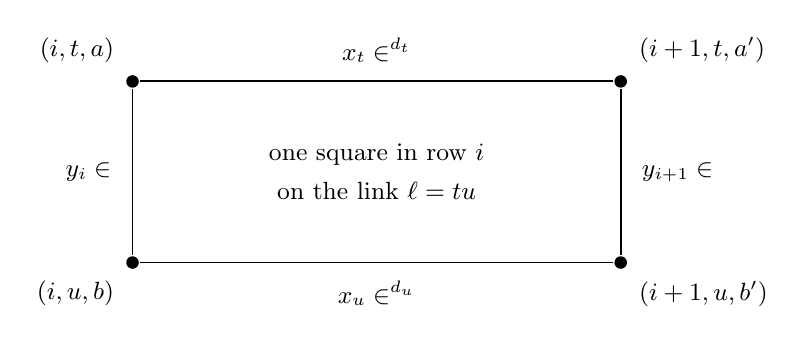
\begin{tikzpicture}[x=1cm,y=1cm,line width=.7pt,font=\small]
 \node[circle,fill,inner sep=1.6pt] (tl) at (0,0) {};
 \node[circle,fill,inner sep=1.6pt] (tr) at (6.2,0) {};
 \node[circle,fill,inner sep=1.6pt] (bl) at (0,-2.3) {};
 \node[circle,fill,inner sep=1.6pt] (br) at (6.2,-2.3) {};
 \draw (tl) -- node[above=3pt] {\(x_t\in\F^{d_t}\)} (tr);
 \draw (bl) -- node[below=3pt] {\(x_u\in\F^{d_u}\)} (br);
 \draw (tl) -- node[left=4pt] {\(y_i\in\F\)} (bl);
 \draw (tr) -- node[right=4pt] {\(y_{i+1}\in\F\)} (br);
 \node[above left=3pt] at (tl) {\((i,t,a)\)};
 \node[above right=3pt] at (tr) {\((i+1,t,a')\)};
 \node[below left=3pt] at (bl) {\((i,u,b)\)};
 \node[below right=3pt] at (br) {\((i+1,u,b')\)};
 \node[align=center] at (3.1,-1.15)
   {one square in row \(i\)\\[3pt]on the link \(\ell=tu\)};
\end{tikzpicture}
\caption{The corner diagram of a single square. The side labels satisfy
\((a,b)\in\cM_{\ell,i}\) and
\((a',b')\in\cM_{\ell,i+1}\). The horizontal readouts are vector-valued;
the vertical readouts are scalar.
These corners belong to the affine data; the output-graph vertices are
introduced in the next section.}
\label{offset:fig-square}
\end{figure}


\subsection{The extension target and a site-ring model}

The block translations needed in the game must preserve every offset
already chosen, while permitting one more block to be added. The following
statement gives that extension property together with closure under
discarding blocks. Its proof occupies the rest of this section.

\begin{proposition}[Compatible offsets with exact projection]
\label{prop:exact-projection}
If the product scalar-image instance is consistent, there are nonempty
families \(\cH_U\), for every \(U\subseteq\cB\) with \(\abs{U}\le K\),
of lists
\[
  \boldsymbol\xi=(\xi_B)_{B\in U},\qquad \xi_B\in\cZ_B^1,
\]
such that the offsets within a list agree on every shared readout and
\begin{equation}
       \cH_U|_V=\cH_V
       \qquad\text{whenever }V\subseteq U.
       \label{eq:exact-projection}
\end{equation}
Here restriction deletes the entries belonging to \(U\setminus V\).
\end{proposition}

The families select suitable compatible lists; every list in a smaller
family must extend to each permitted larger block set.

A ring of sites illustrates how closing a cycle can constrain a shift
in this extension problem. Fix a type \(t\) and an allowed address
\(\mathbf a\in\prod_{i=1}^r A_{t,i}\). The \(r\) site blocks with
readouts \(x_i=x_{i,t,a_i,a_{i+1}}\) form a cycle on the corners
\((i,t,a_i)\). For this model, choose vectors
\(M_1,\ldots,M_r,h\in\F^{d_t}\), set \(M_{r+1}=M_1\), and write
\[
             x_i=M_i+M_{i+1}+\delta_i h.
\]
Every potential \(M_i\) occurs twice in the ring sum. Since only
\(\delta_r\) is nonzero,
\[
                         \sum_{i=1}^r x_i=h.
\]
Thus the complete ring determines the shift \(h\). Conversely, if
this equality holds, choosing \(M_1\) and solving successively around
the cycle gives potentials realizing all the \(x_i\).

After one site is deleted, the retained edges form a path. For any
new shift \(\widetilde h\), its potentials can be solved successively
along that path while all retained \(x_i\) stay fixed. The missing
edge removes the ring-sum constraint. Put \(g=\widetilde h+h\).
Figure~\ref{fig:projection-gauge} shows one such adjustment.
The general proof must handle squares,
partial address domains, and several components that merge when a
block is added. The next two lemmas generalize the cycle distinction:
a closed walk that crosses the row-\(r\) seam an odd number of times
needs at least \(r\) blocks, and with exactly \(r\) it determines a
full address. On components without such a walk, a later potential
adjustment preserves all retained readouts.

\begin{figure}[tbp]
\centering
\begin{minipage}[t]{0.47\linewidth}
\centering
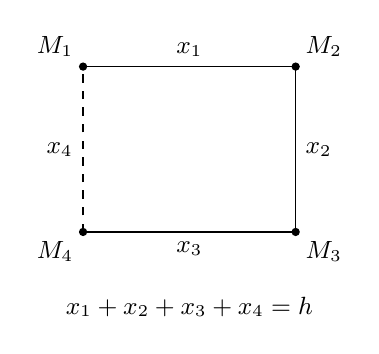
\begin{tikzpicture}[font=\small,line width=0.5pt]
 \coordinate (v1) at (0,0);
 \coordinate (v2) at (2.7,0);
 \coordinate (v3) at (2.7,-2.1);
 \coordinate (v4) at (0,-2.1);
 \draw (v1)--node[above]{$x_1$}(v2)
       --node[right]{$x_2$}(v3)
       --node[below]{$x_3$}(v4);
 \draw[dashed,thick] (v4)--node[left]{$x_4$}(v1);
 \foreach \v in {v1,v2,v3,v4} \fill (\v) circle (1.5pt);
 \node[above left] at (v1) {$M_1$};
 \node[above right] at (v2) {$M_2$};
 \node[below right] at (v3) {$M_3$};
 \node[below left] at (v4) {$M_4$};
 \node at (1.35,-3.05) {$x_1+x_2+x_3+x_4=h$};
\end{tikzpicture}
\end{minipage}\hfill
\begin{minipage}[t]{0.50\linewidth}
\centering
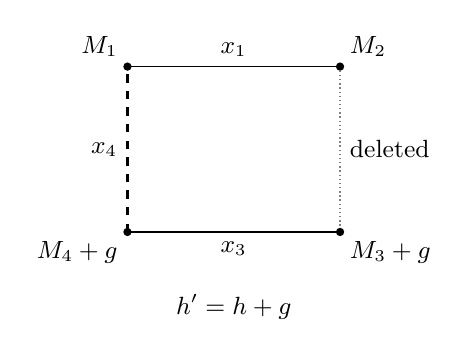
\begin{tikzpicture}[font=\small,line width=0.5pt]
 \coordinate (v1) at (0,0);
 \coordinate (v2) at (2.7,0);
 \coordinate (v3) at (2.7,-2.1);
 \coordinate (v4) at (0,-2.1);
 \draw (v1)--node[above]{$x_1$}(v2);
 \draw[densely dotted,gray] (v2)--node[right,text=black]{deleted}(v3);
 \draw (v3)--node[below]{$x_3$}(v4);
 \draw[dashed,thick] (v4)--node[left]{$x_4$}(v1);
 \foreach \v in {v1,v2,v3,v4} \fill (\v) circle (1.5pt);
 \node[above left] at (v1) {$M_1$};
 \node[above right] at (v2) {$M_2$};
 \node[below right] at (v3) {$M_3+g$};
 \node[below left] at (v4) {$M_4+g$};
 \node[align=center] at (1.35,-3.05)
   {$h'=h+g$};
\end{tikzpicture}
\end{minipage}
\caption{A site ring and the potential adjustment at one type and
one address, with $r=4$.  The dashed edge is the row-$4$ seam.
Left: every potential occurs twice in the sum, leaving $h$.
Right: after deleting row $2$, changing $h$ to $h+g$ and adding $g$
to $M_3,M_4$ preserves every retained readout.  The dotted segment
is absent from the retained corner graph.  The general proof uses
\Cref{offset:lem-gauge} on any nonwrapping component,
not only a cut site ring.}
\label{fig:projection-gauge}
\end{figure}


\subsection{Small supports and recovered addresses}
\label{offset:small-supports}

For \(U\subseteq\cB\), let \(\Gamma_U\) be the union of the corner
diagrams of its blocks. Shared corners and shared named edges are
identified. A block belongs wholly to one connected component of
\(\Gamma_U\). The \emph{support} of a component is its set of types and
its set of distinct wire links: horizontals stay at one type, whereas
verticals project to their links. In particular, several squares on the
same link do not create several support edges.
Write \(\mathcal T(C)\) for the set of types in the support of \(C\).

\begin{lemma}[Small supports]
\label{offset:lem-support}
If \(\abs{U}\le K\), the support of every component of \(\Gamma_U\) is a
tree with at most one real type. Without a real type, it lies in the
interior of a single wire. With a real type, it consists of that type
and possibly initial arms of wires incident with it.
\end{lemma}

\begin{proof}
The support is connected because the corner component is connected.
Only square blocks introduce support links, so it has at most
\(\abs{U}\le K\) distinct links. Internal wire types are private and have
degree two in the full wire layout. A path connecting distinct real
types, or a cycle in that layout, must therefore contain a whole wire,
which has \(4K+1>K\) links. Neither can occur in this support.
This also excludes a cycle created by a loop schema or by parallel
schemas. The stated descriptions follow by following the private wire
interiors from the unique real type, if one is present.
\end{proof}

For every coordinate of every oriented link, fix a permutation
\(\pi_{\ell,i}\) of the ambient label set \(\{0,1\}\) that extends its
matches. Such a permutation exists because those matches are the graph
of an injection on a nonempty binary subset. Use the identity for
identity matches, including partial identities, and use
\(\pi_{\ell,i}^{-1}\) in the reverse direction. These permutations are
analytical choices; actual vertical edges still use only actual matches.

In a support tree, fix a reference type. Unique paths transport the
ambient labels at each type to the reference, separately at each
coordinate. We call the transported labels \emph{aligned labels}.
Every vertical edge preserves its aligned label. Changing the reference
applies the same coordinate permutation to all labels, and restricting
to a subtree gives the same alignment up to this change of reference.
Consequently an aligned binary address can be expressed at any type in
the support. Its expression at an internal type need not satisfy that
wire's full address domain unless a further argument supplies this fact.

Assign a marker \(\omega\in\F\) to each named edge: a horizontal in row
\(i\) has marker \(\delta_i\), and a vertical has marker zero.
A collection of blocks, or a corner component, is \emph{wrapping} if its
diagram contains a closed walk whose marker sum is one. Traversals,
including repeated traversals, are counted in this sum.

\begin{lemma}[Wrapping and address recovery]
\label{offset:lem-wrapping}
Let \(\abs{U}\le r+1\).
\begin{enumerate}
 \item Every wrapping subcollection of \(U\) has at least \(r\) blocks.
 \item A wrapping subcollection with exactly \(r\) blocks has one block
 in each row, lies in a single corner component, and determines a unique
 full aligned address.
 \item Any two wrapping \(r\)-block subcollections of \(U\) lie in the
 same corner component and determine the same address in that
 component's alignment.
 \item If the support of a wrapping \(r\)-block subcollection has no real
 type, it lies in a single wire \(e\), and its recovered address,
 expressed in that wire's internal labels, belongs to \(A_e\).
\end{enumerate}
\end{lemma}

\begin{proof}
Take a marker-one closed walk. Let \(c_i\in\F\) be the parity of its
horizontal traversals in row \(i\). Counting incidences at all corners
on boundary \(i\) gives
\[
 c_{i-1}+c_i=0.
\]
Indeed, the total incidence count of a closed walk at those corners is
even, and a vertical traversal contributes twice on the same boundary.
Since the marker sum is \(c_r=1\), all \(c_i\) equal one. Each row
therefore contributes a horizontal edge to the walk, and every block
has horizontals in just one row. This proves the first assertion.

With exactly \(r\) blocks, there must be one block in every row.
The witness walk meets all of them, so all lie in its corner component.
Use the alignment of that component, or of any containing corner
component in \(\Gamma_U\). The horizontals of the unique row-\(i\)
block prescribe one aligned label at boundary \(i\) and one at boundary
\(i+1\): for a square the two horizontals have the same aligned labels
because of its vertical matches.

Now count incidences at boundary \(i\) separately for each aligned label.
Vertical traversals contribute an even number of incidences to that
label. The total horizontal contribution from each neighboring row is
odd and occurs at that row's prescribed label. The labels prescribed
by rows \(i-1\) and \(i\) must therefore agree. Their common value is the
\(i\)-th coordinate of the recovered address. This proves existence and
uniqueness.

Two \(r\)-element subcollections of a set of size at most \(r+1\) share
at least \(r-1\) blocks. In the present setting these common blocks have
distinct rows. In particular, the two subcollections are in the same
corner component. Every boundary is incident with a common row, since
at most one row is missing from the overlap and \(r\ge3\). Its address
coordinate is consequently the same for both subcollections.

Finally, a support without a real type is inside one wire by
\Cref{offset:lem-support}. All its internal matches are identities.
Every recovered coordinate is the label of a corner at an internal
type, and hence lies in \(A_{e,i}\). Reading all coordinates gives an
address in \(A_e\).
\end{proof}

Only wrapping subcollections of exactly \(r\) blocks will select an
address in the construction below. A component with \(r+1\) blocks may
wrap without containing such a subcollection; no address condition will
be imposed on that component.

\subsection{Admissible shifts and corner potentials}
\label{offset:shifts}

Suppose now that the scalar-image instance is consistent, and fix
nonempty witnesses \(Q_{P,\mathbf a}\) satisfying
\Cref{eq:scalar-images}. For every wire \(e:P\to R\) and every
\(\mathbf a\in A_e\), define the nonempty scalar set
\begin{equation}
 D_{e,\mathbf a}
   =\phi_{e,0}(Q_{P,\mathbf a})
   =\phi_{e,1}
       (Q_{R,\boldsymbol\sigma_e(\mathbf a)}).
 \label{offset:eq-wire-images}
\end{equation}
These are individual image equalities, with no requirement on joint
images of different forms.

Fix \(U\subseteq\cB\) with \(\abs{U}\le K\), and a component \(C\) of
\(\Gamma_U\). A \emph{shift system} on \(C\) is a vector
\[
 (h_t)_{t\in\mathcal T(C)},\qquad h_t\in\F^{d_t},
\]
satisfying \Cref{eq:link-equation} on every support link. Its coordinates
are indexed by the types of this component: different corner components
may use different shifts at the same type.

We call the shift system \emph{admissible} if it also satisfies the
following condition whenever \(C\) contains a wrapping \(r\)-block
subcollection. By \Cref{offset:lem-wrapping}, the recovered address is
independent of that subcollection.
\begin{itemize}
 \item If the support contains a real type \(P\), express the recovered
 address there as \(\mathbf a_P\), and require
 \(h_P\in Q_{P,\mathbf a_P}\).
 \item If the support has no real type, let \(e\) be its wire, express the
 recovered address in the internal labels as \(\mathbf a\), and require
 the common internal scalar to belong to \(D_{e,\mathbf a}\).
 The address lies in \(A_e\) by \Cref{offset:lem-wrapping}.
\end{itemize}
If \(C\) contains no wrapping \(r\)-block subcollection, there is no
additional condition. Write \(\mathcal S(C)\) for the set of admissible
shift systems.

\begin{lemma}[Existence of shifts]
\label{offset:lem-shifts-exist}
Every set \(\mathcal S(C)\) just defined is nonempty.
\end{lemma}

\begin{proof}
If the support has no real type, all its types lie in one wire interior.
Its equations merely identify their scalar shifts. Choose any scalar,
or any element of \(D_{e,\mathbf a}\) when that condition is present.
If the support has a real type \(P\), choose any vector in
\(\F^{d_P}\), or any vector of \(Q_{P,\mathbf a_P}\) when required.
The endpoint equation then determines the scalar along each incident
arm, and the interior equations propagate it along that arm. The arms
do not meet, so there is no further compatibility requirement.
\end{proof}

In particular, when a real type is present we do not additionally impose
an image-set condition on every arm. Some arm may not admit the
recovered address in its full wire domain. Its shift is nevertheless
well defined by the endpoint equation, which is the only condition
needed there.

Choose independently an admissible shift system on each corner
component. At every corner \(v=(i,t,a)\), choose an arbitrary potential
\(M_v\in\F^{d_t}\). Define values on its component's named edges by
\begin{equation}
\begin{aligned}
 x_{vw}&=M_v+M_w+\delta_i h_t
 &&\text{for a horizontal in row \(i\) at type \(t\)},\\
 y_{vw}&=L_{\ell,t}M_v+L_{\ell,u}M_w
 &&\text{for a vertical on \(\ell=tu\)}.
\end{aligned}
\label{offset:eq-potentials}
\end{equation}
Every square satisfies \Cref{eq:square-equation} with \(\eps=1\).
Indeed, each corner potential occurs twice in its boundary expression
and cancels, leaving
\[
 \delta_i\bigl(L_{\ell,t}h_t+L_{\ell,u}h_u\bigr)
       =\delta_i b_\ell.
\]
Sites have no equation. Since a named edge is assigned only one value,
the resulting offsets agree on all readouts shared between blocks.

Define \(\cH_U\) to be the set of all lists
\[
  \boldsymbol\xi=(\xi_B)_{B\in U},
  \qquad \xi_B\in\cZ_B^1,
\]
obtained in this way from admissible shifts and arbitrary corner
potentials. The shifts exist by \Cref{offset:lem-shifts-exist}, so
\(\cH_U\) is nonempty. For \(U=\varnothing\), it consists of the empty
list. We make no uniqueness claim for representations by shifts and
potentials; all permitted representations contribute to the same family.

\subsection{Restriction and extension}
\label{offset:restriction}

Two lemmas isolate the roles of wrapping and nonwrapping components.
The first concerns the shifts themselves, whereas the second permits
shifts to change while preserving the represented offsets.

\begin{lemma}[Lifting shifts from a wrapping component]
\label{offset:lem-wrapping-lift}
Let \(V\subsetneq U\subseteq\cB\), with \(\abs{U}\le r+1\).
If \(C_0\) is a wrapping component of \(\Gamma_V\), and \(C\) is its
containing component in \(\Gamma_U\), restriction of shift systems defines
a surjection
\[
    \mathcal S(C)\longrightarrow\mathcal S(C_0).
\]
\end{lemma}

\begin{proof}
We have \(\abs{V}\le r\). By \Cref{offset:lem-wrapping}, \(C_0\) uses
exactly \(r\) blocks. Its recovered address is the one used for \(C\),
expressed in the respective coordinate systems. There are three cases.

If the support of \(C_0\) contains a real type \(P\), it is also the
unique real type of \(C\). The admissible systems on either component
are parameterized by the same vector \(h_P\in Q_{P,\mathbf a_P}\);
that vector determines the scalars on all of their arms. Restriction
preserves this parameter and is onto.

If the support of \(C\) has no real type, both components are inside the
same wire \(e\). Their admissible systems are parameterized by the same
scalar in \(D_{e,\mathbf a}\), so restriction is again onto.

In the remaining case, \(C\) contains a real type \(P\), but \(C_0\) does
not. The connected support of \(C_0\) lies inside one arm at \(P\),
belonging to a wire \(e\). Its recovered internal address
\(\mathbf a\) belongs to \(A_e\). Therefore the ambient permutation
transport from that address to the incident real endpoint agrees, on
every coordinate, with the actual endpoint map: it is the identity if
\(P\) is the first endpoint, and \(\boldsymbol\sigma_e\) if \(P\) is the
second. Thus the map from the parameter for \(C\) to the parameter for
\(C_0\) is respectively
\[
 \phi_{e,0}:Q_{P,\mathbf a}\longrightarrow D_{e,\mathbf a},
 \qquad\text{or}\qquad
 \phi_{e,1}:Q_{P,\boldsymbol\sigma_e(\mathbf a)}
                    \longrightarrow D_{e,\mathbf a}.
\]
The applicable map is onto by \Cref{offset:eq-wire-images}.
Once its preimage has been chosen, all the other arm scalars of \(C\)
are determined and admissible. Only the incident endpoint of this arm
is used, so the argument also covers a loop wire. Injectivity of the
endpoint form is not required.
\end{proof}

\begin{lemma}[Changing shifts on a nonwrapping component]
\label{offset:lem-gauge}
Let \(C_0\) be a nonwrapping corner component. Suppose two shift systems
\((h_t)\) and \((\widetilde h_t)\) satisfy the link equations on its
support. Every collection of offsets represented by the first system
and corner potentials can also be represented by the second system
after changing those potentials.
\end{lemma}

\begin{proof}
Put \(g_t=\widetilde h_t+h_t\). Adding the two copies of the link
equation gives
\begin{equation}
   L_{\ell,t}g_t=L_{\ell,u}g_u
   \quad\text{on every support link }\ell=tu.
   \label{offset:eq-shift-difference}
\end{equation}
Since \(C_0\) is nonwrapping, the marker sum is zero on every closed walk.
Choose one corner as a root, and define \(s_v\in\F\) to be the marker sum
along a path from it to \(v\). This is independent of the path: the
concatenation of two such paths, reversing one, is a closed walk.
Consequently
\[
     s_v+s_w=\omega(vw)
\]
on every named edge.

Replace the old potential at a corner of type \(t\) by
\(\widetilde M_v=M_v+s_vg_t\). On a horizontal in row \(i\), the change
in \Cref{offset:eq-potentials} is
\[
 (s_v+s_w)g_t+\delta_i(\widetilde h_t+h_t)
       =(\delta_i+\delta_i)g_t=0.
\]
On a vertical, \(s_v=s_w\), so the change is
\[
 s_vL_{\ell,t}g_t+s_wL_{\ell,u}g_u=0
\]
by \Cref{offset:eq-shift-difference}. Thus all old readout values are
preserved. The argument allows vector shifts at a two-dimensional
real type and does not require its endpoint forms to be nonzero.
\end{proof}

\begin{proof}[Proof of \Cref{prop:exact-projection}]
Use the families defined by \Cref{offset:eq-potentials}. Nonemptiness,
legality, and agreement on shared readouts have already been proved.
It remains to establish the projection equality. The case \(V=U\)
is immediate, so suppose \(V\subsetneq U\). Then \(\abs{V}\le r\).
Each component \(C_0\) of \(\Gamma_V\) lies in a component \(C\) of
\(\Gamma_U\).

First take a represented list in \(\cH_U\) and restrict its shifts and
potentials to each \(C_0\). These shifts satisfy all old link equations.
If \(C_0\) is nonwrapping, it has no additional address condition.
If it wraps, their admissibility follows from
\Cref{offset:lem-wrapping-lift}. The restricted representation therefore
belongs to \(\cH_V\), proving
\(\cH_U|_V\subseteq\cH_V\).

For the other inclusion, fix an arbitrary list in \(\cH_V\), and choose
any one of its representations by admissible old shifts and potentials.
There is at most one wrapping old component: one would already require
\(r\) of the at most \(r\) old blocks.
For each component \(C\) of \(\Gamma_U\), choose an admissible new shift
system. If \(C\) contains the wrapping old component \(C_0\), choose it
to extend the selected old shifts on \(C_0\), using
\Cref{offset:lem-wrapping-lift}. On all other new components choose any
admissible shifts.

Keep the old potentials on a wrapping old component. On every
nonwrapping old component, apply \Cref{offset:lem-gauge} to replace its
old shifts by the restriction of the chosen new shifts without changing
any old offset. Distinct old components have disjoint corner sets,
so these potential changes coexist even when several old components
merge into a single new component or have different old shifts at the
same type. Assign arbitrary potentials to the additional corners of
\(\Gamma_U\).

The new shifts and these potentials represent a member of \(\cH_U\).
They satisfy every new square equation by
\Cref{offset:eq-potentials}, while on each old named edge the value is
unchanged. Hence this member restricts to the prescribed list in
\(\cH_V\), proving the reverse inclusion.
\end{proof}

There are two useful features of this proof. First, if a component
first becomes wrapping only when all \(r+1\) blocks are present, it has
no wrapping proper subcollection and no address condition is needed:
all the old components are covered by the gauge lemma. Second, a
wrapping old component asks for at most one scalar preimage from a
real-type witness set. Thus the individual image equalities in
\Cref{offset:eq-wire-images} suffice, even for non-affine witness sets
or noninjective endpoint forms. The families \(\cH_U\), their shifts,
and the witnesses \(Q_{P,\mathbf a}\) are used only in this existence
argument; the reduction never enumerates them.
